\documentclass[a4j, twocolumn]{jarticle}

\usepackage[dvipdfmx]{graphicx}
\usepackage{caption}
\usepackage{subcaption}

\begin{document}

\title{ゴルフについての基礎知識}
\author{イマムカイリルビス\thanks{釧路工業高等専門学校}}
\date{\today}

\maketitle

\section{ゴルフの誕生}

世界のスポーツの中でも,最も古い歴史を持つといっても通信できないのが,”ゴルフ”である.そして,長い歴史を持っているために,その起源いまだに謎に包まれている.最も有力とされるのは,スコットランドの羊飼いが先の曲がった杖で小石や羊の糞を打ち,ウサギの巣穴へ入れて遊んだのがゴルフにつながったとういう訳である.15世紀にすでにゴルフが広く多くの人たちの間で楽しまれていた.しかし,
\begin{itemize}
    \item 兵士がゴルフに夢中になり,訓練をおそらかにしたため,イングランドの戦争に負けた.
    \item 国民の多くがゴルフばかりしていて働かなくなった.
\end{itemize}
などの理由から,1457年,スコットランド王ジェームス2世が,第14会議で「フットボールとゴルフは絶対禁止しなくてはならない.」という,「ゴルフ禁止令」を発令したという記事が残っている.\cite{bib1}\\

\vspace{-15pt}

その後,数回にわたり,「ゴルフ禁止令」が発令された.しかし,1502年当時の国王ジェームス4世は,自分はゴルフをしたかったために,このゴルフ禁止令を解除した.そして,人々は再びゴルフを楽しむようになったのである.お隣のイングランドへも,この頃にゴルフを伝わったとされている.\cite{bib1}\\

\section{ゴルフの道具}

ゴルフをするにはなんといってもクラブとボールがなければ始まらない.クラブとボールの規格はルールで厳しく制限され,選手は14本のクラブまで使用してよいことになっている.\cite{bib2}.このクラブセッティングが選手の成績に大きく影響する.表1,2に主なクラブの名称,飛距離などを記述する.

\begin{table}[htb]
    \caption{ウッドの種類}
    \label{Wood_Table}
    \vspace{-7.0mm}
    \begin{center}
        \begin{tabular}{|c|c|c|}
            \hline
            \multicolumn{3}{|c|}{ウッド(Wood)}\\ %ini harusnya box
            \hline
            \multicolumn{3}{c}{}\\ [-3.0ex]
            \hline
            番手&名称&飛距離\\
            \hline
            1番&ドライバ&300\\ 
            \hline
            2番&ブラッシ&280\\
            \hline
            3番&スプーン&270\\
            \hline
            4番&バッフィ&260\\
            \hline
            5番&クリーク&250\\
            \hline
        \end{tabular}
    \end{center}
\end{table}
\vspace{-20pt}
\begin{table}[htb]
    \caption{アイアンの種類}
    \label{Iron_Table}
    \vspace{-7.0mm}
    \begin{center}
        \begin{tabular}{|c|c|c|}
            \hline
            \multicolumn{3}{|c|}{アイアン(Iron)}\\
            \hline
            \multicolumn{3}{c}{}\\ [-3.0ex]
            \hline
            番手&名称&飛距離\\ 
            \hline
            1番&ドライビングアイアン&250\\
            \hline
            2番&ミッドアイアン&240\\
            \hline
            3番&ミッドマッシー&230\\ 
            \hline
            4番&マッシーアイアン&220\\
            \hline
            5番&マッシー&210\\
            \hline
            6番&スペードマッシー&200\\
            \hline
            7番&マッシー二ブリック&190\\
            \hline
            8番&ピッチング二ブリック&180\\
            \hline
            9番&二ブリック&170\\
            \hline
        \end{tabular}
    \end{center}
\end{table}

\begin{description}
    \item[ドライバー]
    その音,材質に柿木(パーシモン)を使用していたことからウッド(Wood)とも呼ばれている.芯にあたったときは大きな距離がでるが,その反面左右に曲がりやすい.

    \item[フェアウエイウッド]
    ドライバー以外のウッド,最近はアイアンの代わりに利用するゴルファーも多い,片山晋悟がフェアウエイウッドの名手とされている.しかし,ちょっとジジくさい.

    \item[アイアン]
    文字通り鉄(iron)でできている.アイアンといってもステンレス,チタンなど固くて軽い材料が利用されている.1番から9番まで番手があるが,アマチュアは1,2,3番アイアンは難しくて使えない.アイアンは距離を合わせる場合やグリーンを狙うに使われる.

    \item[ウエッジ]
    主にグリーン周りやバンカーに入った球を打つときに使う.距離が出ないが,弾道が高く球が止まりやすい性質がある.ウエッジブランドではボーケイ等が有名.

    \item[パター]
    グリーンに乗った球をカップに沈めるときに使う.とにかくセンスが必要.この一打で優勝の行方が変わる.
\end{description}

\section{ドライバーの飛距離}

ドライバーの飛距離はトッププロだと300ヤードを楽に超える.飛距離はヘッドスピードとクラブの反発係数に依存する.距離を$D$,ヘッドスピードを$S$,打ち出し角度を$\theta$,クラブの反発係数を$R$とすると(\ref{eq1})式のような関係式が成り立つ~\cite{bib2}\\
\begin{equation}
    \label{eq1}
    D = \frac{R \cdot S^2}{log_e 132}\sin\theta
\end{equation}

ちなみに,(\ref{eq1})式は超テキトーである.

\section{四大メジャーと期待選手}

ゴルフの名誉ある最大規模の大会として以下の四大メジャートーナメントがある.これらのトーナメントを制してはじめて超一流の称号を与えられる.賞金も凄いが,その名誉となると金銭には変わらない価値がある.\\

\vspace{-15pt}

\begin{enumerate}
    \item マスターズ
    \item 全英オープン
    \item 全米オープン
    \item 全米プロ選手権
\end{enumerate}

図~\ref{tigerimg}にタイガーウッズ(48歳)の写真を掲載する.これまでに,4大メジャー大会を15回制覇し,PGA賞金王には10度輝いている.一時期,調子を落とし,2008年以降,メジャー大会での優勝からは遠ざかってしまっていたが,2019年のマスターズで復活優勝を果たした.今年のマスターズも,持病の影響からスコアを落とし,決勝トーナメントへ進出にはならなかった.\\

\begin{figure}[htb]
    \begin{center}
        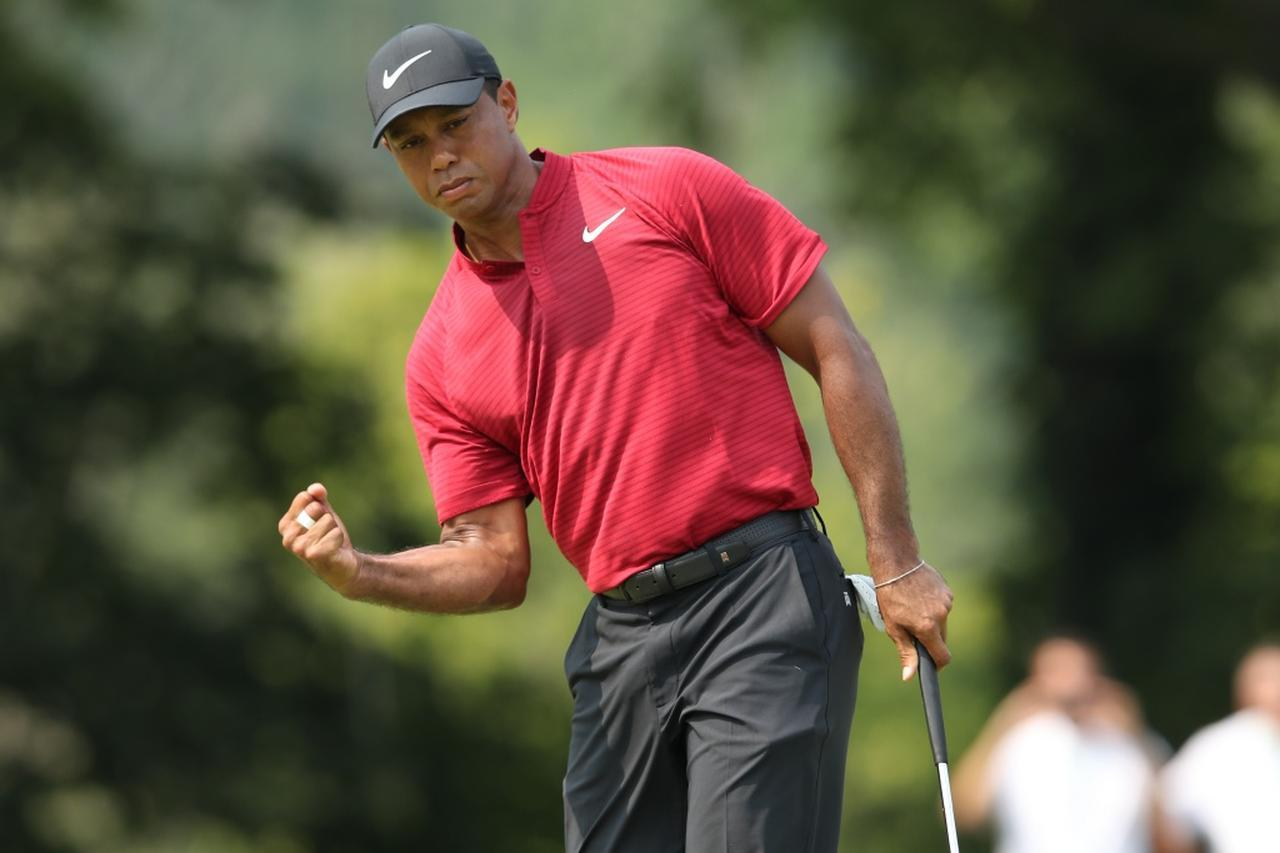
\includegraphics[scale=0.07]{tiger.jpg}
        \caption{世界の帝王T.ウッズ}
        \label{tigerimg}
    \end{center}
\end{figure}

図~\ref{jpnimg}に活躍を期待される2名の日本人選手を紹介する.\\

\vspace{-15pt}

(a)は日本のホープ松山英樹選手.2021年度のマスターズで逐にアジア人として奇跡の初優勝を飾る.ずっとメジャー戦優勝を期待できる唯一の日本人と期待してはいたが,今でも信じれれないくらいの快挙である.彼はメンタルも強いが,肝心のところでのポカミスがなければ4大メジャ大会制覇も夢でない.\\

\vspace{-15pt}

(b)は女子プロの古江彩佳選手.優勝回数はまだ多くないが,安定した成績で常にランキン上位に位置する実力者である.彼女の特徴は飛距離が全然出ないがコントロールが素晴らしいこと.クラブをぶん回してダイナミックに飛ばす女子プロが多い中で異彩を放つ存在である.

\begin{figure}[htb]
    \centering
    \begin{subfigure}[b]{0.12\textwidth}
        \centering
        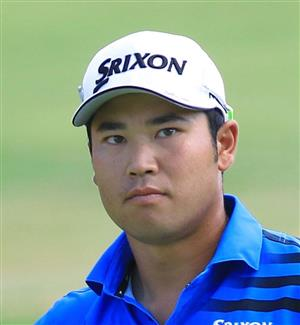
\includegraphics[height=\textwidth]{matuyama.jpg}
        \vspace{-1.0mm}
        \caption{松山英樹}
        \label{matuyamaimg}
    \end{subfigure}
    \begin{subfigure}[b]{0.12\textwidth}
        \centering
        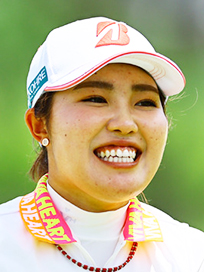
\includegraphics[height=\textwidth]{furue.jpg}
        \vspace{-1.0mm}
        \caption{古江彩佳}
        \label{furueimg}
    \end{subfigure}
        \vspace{-3.0mm}
        \caption{私の期待}
       \label{jpnimg}
\end{figure}

\vspace{-20pt}

\begin{thebibliography}{99}
    \bibitem{bib1}
    穴堀好雄,”俺のゴルフ人生”,OB出版,2016.
    \bibitem{bib2}
    M. Jackson and J. Madonna, "Official Gold Rule", Sport science, 2011.
\end{thebibliography}

\end{document}